\Problem{Presos agressius}

\Statement

Tenim un corredor de presó amb $N$ cel·les situades en posicions diferents d'una recta numè\-rica. Volem col·locar-hi $K$ presos agressius, cadascun en una cel·la diferent.

\medskip

Com que els presos es barallen si estan massa a prop, el director de la presó vol que la distància mínima entre qualsevol parell de presos sigui la màxima possible per garantir la tranquil·litat al corredor.

\medskip
Per exemple, per $N=5$ cel·les situades en les posicions 1 2 4 8 9, si el director vol col·locar-hi 3 presos, la màxima distància mínima possible entre qualsevol parell de presos és 3, que es pot aconseguir col·locant els presos en les cel·les 1, 4 i 9:

\begin{center}
    \begin{latexonly}
    \includegraphics[width=0.75\textwidth]{exemple.pdf}    
    \end{latexonly}
    \begin{htmlonly}
    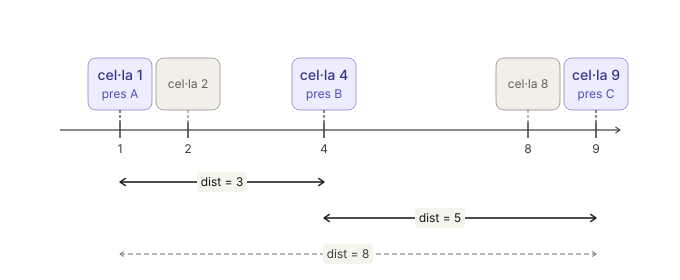
\includegraphics[width=0.75\textwidth]{exemple.svg}    
    \end{htmlonly}
\end{center}

\medskip

Escriviu un programa que, donades les posicions de les cel·les i el nombre de presos,  determini la màxima distància mínima possible entre qualsevol parell de presos col·locats en diferents cel·les.

\Input

Hi ha diversos casos de prova. Cada cas de prova consisteix en dos enters $N$ i $K$ tal que $2 \le K \le N$ seguits de $N$ enters $p_1, p_2, \dots, p_N$, on $p_i$ és la posició de la $i$-èssima cel·la a la recta.

\Output

Per cada cas de prova, imprimiu la màxima distància mínima possible entre qualsevol parell de presos col·locats a les cel·les.

\SampleOneCol

